\chapter{Architecture}
\label{Architecture}
This chapter will give a brief introduction into DXRAM. Then the schema according to which the graphs are going to be loaded will be explained. After that problems that will occure will be discussed. 
\section{DXRAM}
DXRAM is a distrubuted in-memory key/value-store. 
It is implemented in Java and optimized to manage billions of small data objects. 
For low latency data access DXRAM keeps 100\% of the data in RAM.
DXRAM provides a low data overhead, which suits hrapg based application very well.
Nodes of DXRAM can take the role of a "normal" peer or a superpeer. Superpeers are arranged in a chord like ring structure. \begin{figure}[H]
	\centering
	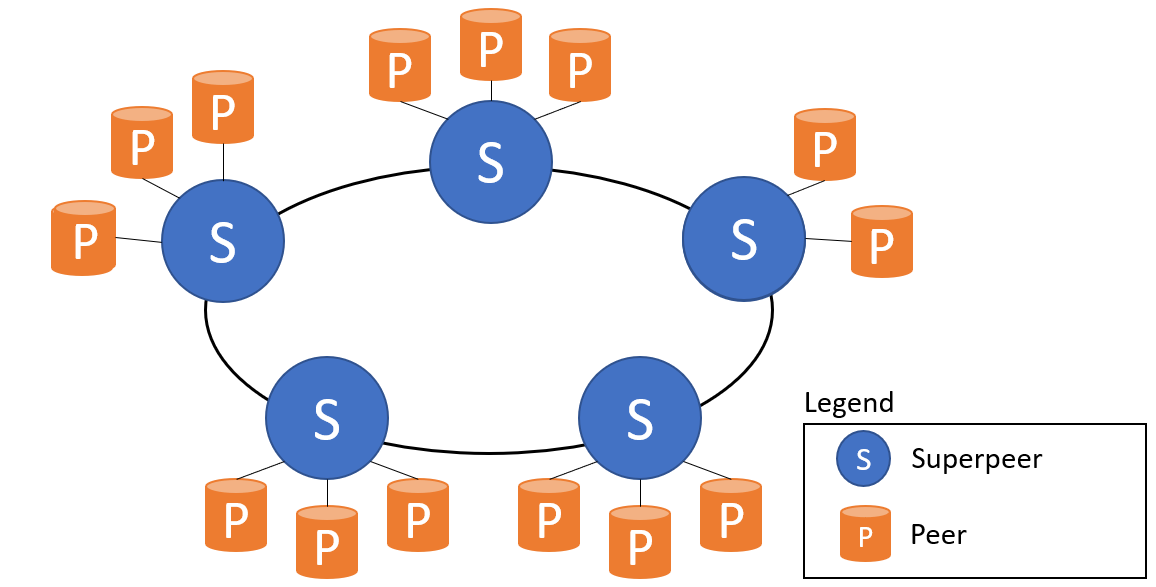
\includegraphics[width=1.0\linewidth]{img/topology.png}
	\caption{Topology of DXRAM}
	\label{topology}
\end{figure}
Peers are always assigned to one superpeer. Superpeer take over adminstativ tasks within the distrubuted system while peers serve the role of a storage or backup nodes.
DXRAM provides its own application programming interface through services.DXRAM uses a distrubuted file system, so every node can access every file. They can be loaded by applications to get access to storage, computing power and more operations. Custom applications can be loaded as jar-files, but must implement the \texttt{AbstractApplication} class and register thereself. All nodes in the system are accessible through the \texttt{BootService}, which can list all online peers and theire role inside the system.
The key/value-store can be accessed by the \texttt{ChunkService}, who provides several operations for creating, getting and storing data structures in chunks. All data structurs, which should be storable, must implement the \texttt{AbstractChunk} class.\\
The computing power of the network can be used in serveral ways. One way is the \texttt{JobService} which manages lightweigth jobs. Every job has a unique id and inherits from \texttt{AbstractJob}. Every job has its own thread and can run on a local nodes or be pushed to a remote node. Job will be pushed into a job queue and wait for their execution.. Another way to compute something is the \texttt{MasterSlaveService} enables to run parallel computations on groups of peers. In this group peers can takes different rolee, one peers takes the role of the master, which coordinates the task. The other peers are either workers(slaves) or take no role. One master and several workers make up one computation group.\cite{Beineke.20180714,dxramoverview}

\subsection{Integration in DXRAM}
There are several ways of integrating foreign code in DXRAM. One goal is to be able to load data via a terminal command, but also to be able to easily integrate the loader as a library. Therefore the main part of the application will be accessible through a custom Job, which can be used as library.\\
To provide terminal access, without the current possibility to execute jobs from the terminal, the job will be wrapped by an DxApp.

\begin{figure}[H]
	\centering
	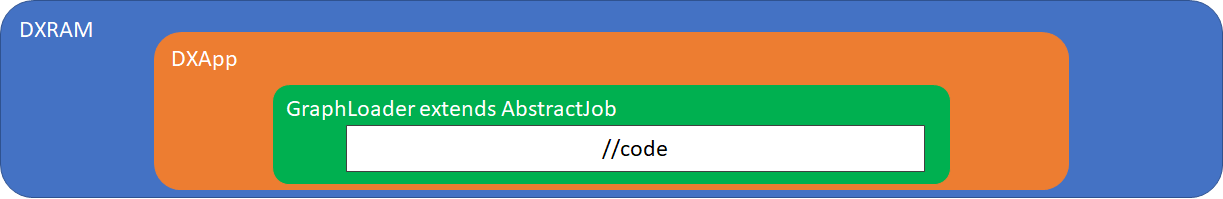
\includegraphics[width=1.0\linewidth]{img/schema.png}
	\caption{Schema of  code integeration in DXRAM}
	\label{topology}
\end{figure}

\section{Architecture of the Application}
The loading of the file formats will be managed in three steps:
\begin{enumerate}
\item Deploying the file in the distributed system 
\item Peers read and load the data of their chunks
\item All loaded data is stored in the key/value-store
\end{enumerate}

First, a basic graph implementation with vertices and edges must be provided, those should be extendable duo to different graphs, vertex and edge requirements of each format and application.
Then the graph file will be split by lines for mostly likly simple graph file formats or interpreted for more complex ones. Out of those file splits - file chunks will be created which will be deployed to the corresponding peer. The peer will run the loading job with the loader provided for the format. The file format will be specified by the user as paramter.

\begin{figure}[H]
	\centering
	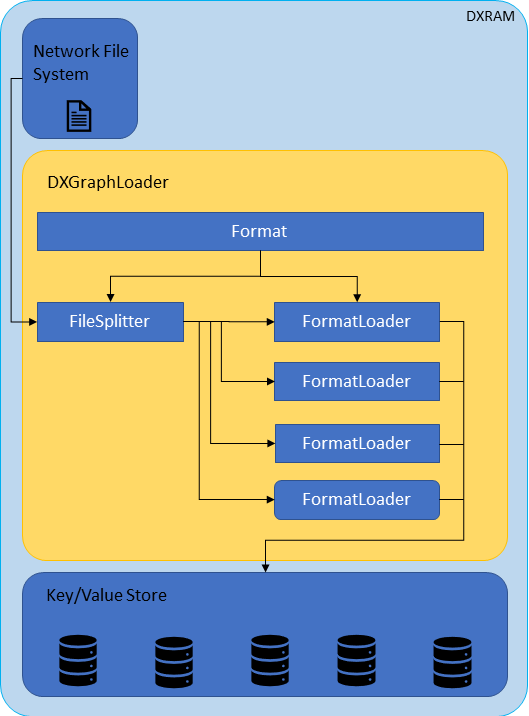
\includegraphics[width=1.0\linewidth]{img/layout.png}
	\caption{Topology of DXRAM}
	\label{topology}
\end{figure}


\subsection{Deployment of File data on nodes}
The deployment can be done in multiple ways, which have to be evaluated. One possibility would splitting the original file into multiple smaller files and access them via the NFS. This approach would be straight forward, but results in one read and write operation of the whole original file size. Also the file would need to be loaded again into memory for extracting its data. This would result in O(2n) on the initiating peer and O(n/chunks).
Another approach would be to load the data into memory and send chunk structures to the according peers. This reduces the writing operation and another reading operation on the peer, because the data lays already in memory.
The last method would be to access the original file via the NFS and extract the chunk directly on the remote peer. This would result in distriubution of the loading of the original file in one run, but could result in the bottleneck of the one storing node with the original file. This would probably be slower duo to the fact that all nodes accessing one file, would cause a random read sequence, which is often slower then sequential reads.

\subsubsection{Efficient Loading of File into Memory}
One key ability of the application is that the loading of the file system should be fast. Often the reading/writing from Storage Devices is a bottleneck. The first problem is that most Storage Devices are designed for sequential read and write operations and often support only one operation at a time. This leads to the problem that multiple threads reading the storage device is a waste of performance and won’t speed up the input rate of the file. Another problem is that accessing a storage device will cause a context switch. This results in the application stopping, while the kernel executes sensitive functions. This problem is often address with buffering the files and by requesting more data then needed in one step. Buffer sizes are one optimization problem to consider. [5]\\
The traditional way of accessing the data of a file is a common routine. First the file gets opened after that the data can be read, written in sequential or random order. This method causes many context switches, which force the application to stop, while the kernel executes sensitive functions. That’s why in nearly every case IO gets buffered, so the context switches occur less often. [6]\\
To reduce the amount of context switches to a minimum. This problem is addressed by memory mapping and suits large files where we can reduce the context switches drastically. A virtual memory mapping between the filesystem and the application address space is created. So expansive system calls can be avoided. The setup of this method is more expensive then the setup of file IO. [5,6]\pageref{sec:FileReading}


\subsection{Processing/Parsing of the Data}
The processing/ parsing of the data is unique for each format. Some formats like the TGF need a a different parser in contrast to XML or JSON sytle formats. The best option would be to create as many threads as possible to read in the data.

\subsection{Storing}
The extracted vertices, edges and optional metadata needs to be stored. For this task the \texttt{ChunkService} will be used to push the created structs into the key/value-store. ne problem of the distrubuted loading is that peers cannot wait on other peers to get information about vertices, because this would result in too much messages and network traffic for large datasets. This still leaves the problem of not synchronized vertex objects on different peers, which cant be written to the key/value-store because their information could be incomplete. 
\subsubsection{Duplicate node objects}
Some formats (especially in edge lists) nodes just get described by their edges. One problem is if two different peers create the same nodes by different edges, so they don’t know if other peers already created a node object for specific nodes. As result they create a local node object with the information they got. In that case after reading the file in its entirety some merge of all hash maps and objects would need to be done. This would result in the problem that one assumption of this work is that one peer can’t keep all nodes and edges in memory, because there are too many objects.\\
Hash-Distribution of the Nodes while reading\\
As result of the fact of reorganizing the nodes after they have been loaded is very inefficient and doesn’t suit our needs, the next approach would be to organize the nodes at loading/parsing-time.
One way could be to hash the labels/ids used in the graph. Note that the hashes created have no security constrains and don’t need to be unique. This hash could be used to divide the nodes onto the peers. As result every peer would buffer all nodes, that don’t belong to its range of hash values, and send the information he gathered to the according peers. This way we don’t have to deal with duplicate nodes or merge. One problem of this approach is, that peers could end up with a chunk, that contains no nodes that hash to itself.\\
Hash-Distribution after reading\\
The peers could finish reading the nodes of its chunk and create their own versions in their key-value store. After reading and parsing is finished, they could like in first solution send the key-value-objects to the according nodes based on the hashes of their ids. The target peer then merges all versions of that node and stores the copy that has all information, the other duplicates get deleted. This could result in many objects for one node for each peer

\section{Issues}
A requirement is that the file is located inside one of our peer’s storage devices and isn’t part of our distributed system in any way. Loading files via an internet connection, will not be featured. Some start parameters are indispensable for this type of application, like the absolute file path, the format of the file or rather the parser that should be used and the number of peers to load the file.
Frist one peer should deal with the file, to distribute it to our others peers. The best thing would be, if the peer, who deals with file, would be the same peer where the file is located on. Otherwise the file transfer to the according peer would be a waste of time, especially for file sizes of several gigabytes. After the file chunks got deployed on the network, they could be parsed and loaded by the prior assigned peers into our DXRAM key-value store. [4]


First the file data gets loaded into small chunks which can be distrubted tFirst the file gets partially mapped into the memory, where it can be read by the master slave. The master slave first deals with the format specifications of the file, providing the division schema for splitting the file into chunks. chunks and will be dealing with the file format. Duo to the fact that the data, is in memory, multiple thread can access the data parallel to accelerate processing. The processed data will be collected in chunks which will be deployed to the assigned slaves.
The support of infiniband would be increasing the performance drastically, due to spreading the data in the distributed system would be faster.
When the chunks arrive on the according slaves, they could immediately start processing their chunks.
 
Duo to fact that some formats specify data of nodes in two or multiple places inside the file, it would be an interesting approach of using for example two memory maps of the same file in different sections. So, the chunk (buffer) can be filled with both information at the same time and the node information lie on all on one slave.

